\documentclass[10pt,aspectratio=169]{beamer}

\usepackage[utf8]{inputenc}
\usepackage{kotex}
\usepackage{amsmath,amssymb}
\usepackage{graphicx}
\usepackage{booktabs}
\usepackage{hyperref}

\usetheme{Madrid}
\usecolortheme{default}
\definecolor{NavyDark}{HTML}{0F2027}
\definecolor{NavyMedium}{HTML}{203A43}
\definecolor{TealAccent}{HTML}{10AC84}
\definecolor{OrangeAccent}{HTML}{E67E22}
\definecolor{BgLight}{HTML}{F8F9FA}
\setbeamercolor{palette primary}{bg=NavyDark,fg=white}
\setbeamercolor{palette secondary}{bg=NavyMedium,fg=white}
\setbeamercolor{palette tertiary}{bg=NavyDark,fg=white}
\setbeamercolor{titlelike}{bg=NavyDark,fg=white}
\setbeamercolor{structure}{fg=NavyMedium}
\setbeamercolor{block title}{bg=NavyMedium,fg=white}
\setbeamercolor{block body}{bg=BgLight,fg=black}
\setbeamerfont{title}{size=\large,series=\bfseries}
\setbeamerfont{frametitle}{size=\large,series=\bfseries}
\setbeamertemplate{navigation symbols}{}
\hypersetup{colorlinks=true,urlcolor=TealAccent}

\title[Chameleon Screening Dynamics]{Physical Laws that Hide like a Chameleon}
\subtitle{Density-dependent fifth-force dynamics: revised and verified numerical study}
\author[Dongkyu Lee]{이동규}
\institute[서울대학교]{서울대학교 물리천문학부 물리학전공}
\date{2026년 7월 수정·검증판}

\begin{document}

\begin{frame}[plain]
 \titlepage
\end{frame}

\begin{frame}{1. 핵심 질문: 장의 질량은 왜 환경에 따라 바뀌는가?}
 \begin{columns}[T]
  \begin{column}{0.56\textwidth}
   \begin{block}{유효 포텐셜}
    \[
     V_{\mathrm{eff}}(\phi)=\frac{M^{4+n}}{\phi^n}
     +\rho\,e^{\beta\phi/M_{\mathrm{Pl}}}
    \]
    \[
     m_{\mathrm{eff}}^2=V_{\mathrm{eff}}''(\phi_{\min})
    \]
    \[
     \lambda_c=\frac{\hbar}{m_{\mathrm{eff}}c}
     \quad(\hbar=c=1:\ \lambda_c=m_{\mathrm{eff}}^{-1})
    \]
   \end{block}
   \begin{itemize}
    \item 고밀도: $\phi_{\min}\downarrow$, $m_{\mathrm{eff}}\uparrow$, $\lambda_c\downarrow$ \(\Rightarrow\) short range
    \item 저밀도: $\phi_{\min}\uparrow$, $m_{\mathrm{eff}}\downarrow$, $\lambda_c\uparrow$ \(\Rightarrow\) long range
   \end{itemize}
  \end{column}
  \begin{column}{0.40\textwidth}
   \begin{block}{힘과 thin shell}
    \small
    \[
     \mathbf a_5=-Q_{\mathrm{test}}\frac{\beta}{M_{\mathrm{Pl}}}\nabla\phi
    \]
    \[
     Q_{\mathrm{test}}\simeq\min\!\left(3\frac{\Delta R}{R},1\right)
    \]
    벌크 물체는 $Q\ll1$로 스스로 차폐될 수 있지만 작은 원자는 $Q\simeq1$일 수 있다.
   \end{block}
   \vspace{0.3cm}
   \centering\textcolor{TealAccent}{\bfseries 미검출은 ``검증 불가능''과 다르다.}
  \end{column}
 \end{columns}
\end{frame}

\begin{frame}{2. 무차원화: 코드의 $\beta=1$은 물리적 허용점이 아니다}
 \begin{block}{스케일 정의}
  $x=L_0\hat x$, $\phi=\Phi_0\hat\phi$, $\rho=\rho_0\hat\rho$, $t=T_0\hat t$로 두면
  \[
   A=\frac{nM^{4+n}L_0^2}{\Phi_0^{n+2}},\qquad
   B=\frac{\beta\rho_0L_0^2}{M_{\mathrm{Pl}}\Phi_0},\qquad
   C=\frac{\beta\Phi_0T_0^2}{M_{\mathrm{Pl}}L_0^2}.
  \]
 \end{block}
 \begin{columns}[T]
  \begin{column}{0.48\textwidth}
   \begin{block}{본 프로젝트}
    $n=1$, $A=B=C=1$인 \textbf{무차원 toy model}
    \[
     \hat\phi''=-\hat\phi^{-2}+\hat\rho e^{\hat\phi}.
    \]
   \end{block}
  \end{column}
  \begin{column}{0.48\textwidth}
   \begin{alertblock}{해석의 한계}
    실제 허용 여부는 $(M,n,\beta)$, 챔버 형상, 환경 밀도, source/test-body의 $Q$를 함께 정한 뒤 exclusion contour와 비교해야 한다.
   \end{alertblock}
  \end{column}
 \end{columns}
\end{frame}

\begin{frame}{3. 수치 방법: 정적 BVP $\rightarrow$ 힘 보간 $\rightarrow$ 궤도 IVP}
 \begin{columns}[T]
  \begin{column}{0.49\textwidth}
   \begin{block}{Step 1: 장의 경계값 문제}
    \begin{itemize}
     \item $\hat x\in[-20,20]$, 결과 창 $[-12,12]$
     \item $\hat\rho_{\rm high}=10$, $\hat\rho_{\rm low}=0.01$, $\hat w=1.5$
     \item 경계: $\hat\phi(\pm L)=\hat\phi_{\min}(\hat\rho_{\rm edge})$
     \item \texttt{solve\_bvp}: 4차 collocation, 적응 격자, tol $=10^{-6}$
    \end{itemize}
   \end{block}
  \end{column}
  \begin{column}{0.49\textwidth}
   \begin{block}{Step 2: 입자의 초기값 문제}
    \[
     \dot{\hat x}=\hat v,\qquad
     \dot{\hat v}=-0.15\hat x-\frac{d\hat\phi}{d\hat x}
    \]
    Dormand--Prince RK45의 5차/4차 내장해 차이로 국소오차를 추정하고 step을 수락·거부한다.
    \begin{itemize}
     \item rtol $=10^{-9}$, atol $=10^{-11}$
     \item max step $=0.05$
     \item 직접 구현한 고정 간격 RK4와 교차검증
    \end{itemize}
   \end{block}
  \end{column}
 \end{columns}
 \vspace{0.2cm}
 \centering\small Source: \href{https://github.com/Lasqui-Ponto/Mechanics_Term_Project}{github.com/Lasqui-Ponto/Mechanics\_Term\_Project}
\end{frame}

\begin{frame}{4. 코드 검증: 알려진 해와 수렴률을 재현하는가?}
 \centering
 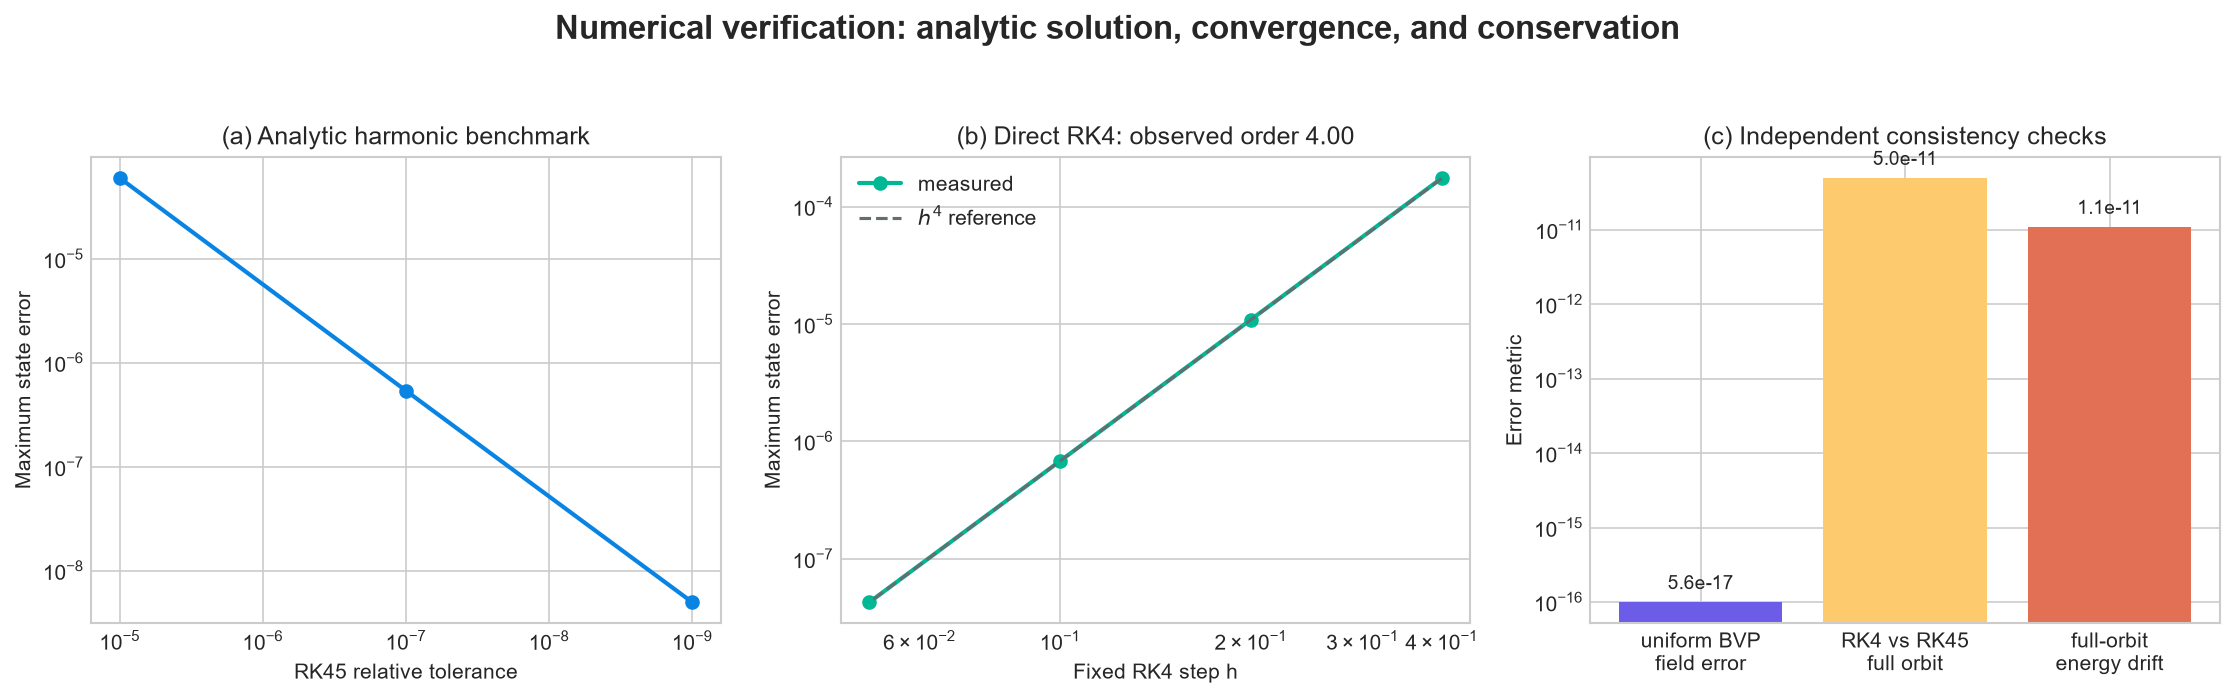
\includegraphics[width=0.91\textwidth]{verification_results.png}
 \vspace{-0.15cm}
 \begin{columns}[T]
  \begin{column}{0.32\textwidth}\centering\scriptsize 조화진동자 해석해와 RK45 비교\end{column}
  \begin{column}{0.32\textwidth}\centering\scriptsize 직접 RK4 관측 차수 $4.0038$\end{column}
  \begin{column}{0.32\textwidth}\centering\scriptsize BVP $5.6\times10^{-17}$; RK4--RK45 $5.0\times10^{-11}$\end{column}
 \end{columns}
\end{frame}

\begin{frame}[shrink=3]{5. 결과 I: 매끄러운 밀도 경계가 보존 궤도를 어떻게 바꾸는가?}
 \begin{columns}[T]
  \begin{column}{0.67\textwidth}
   \centering
   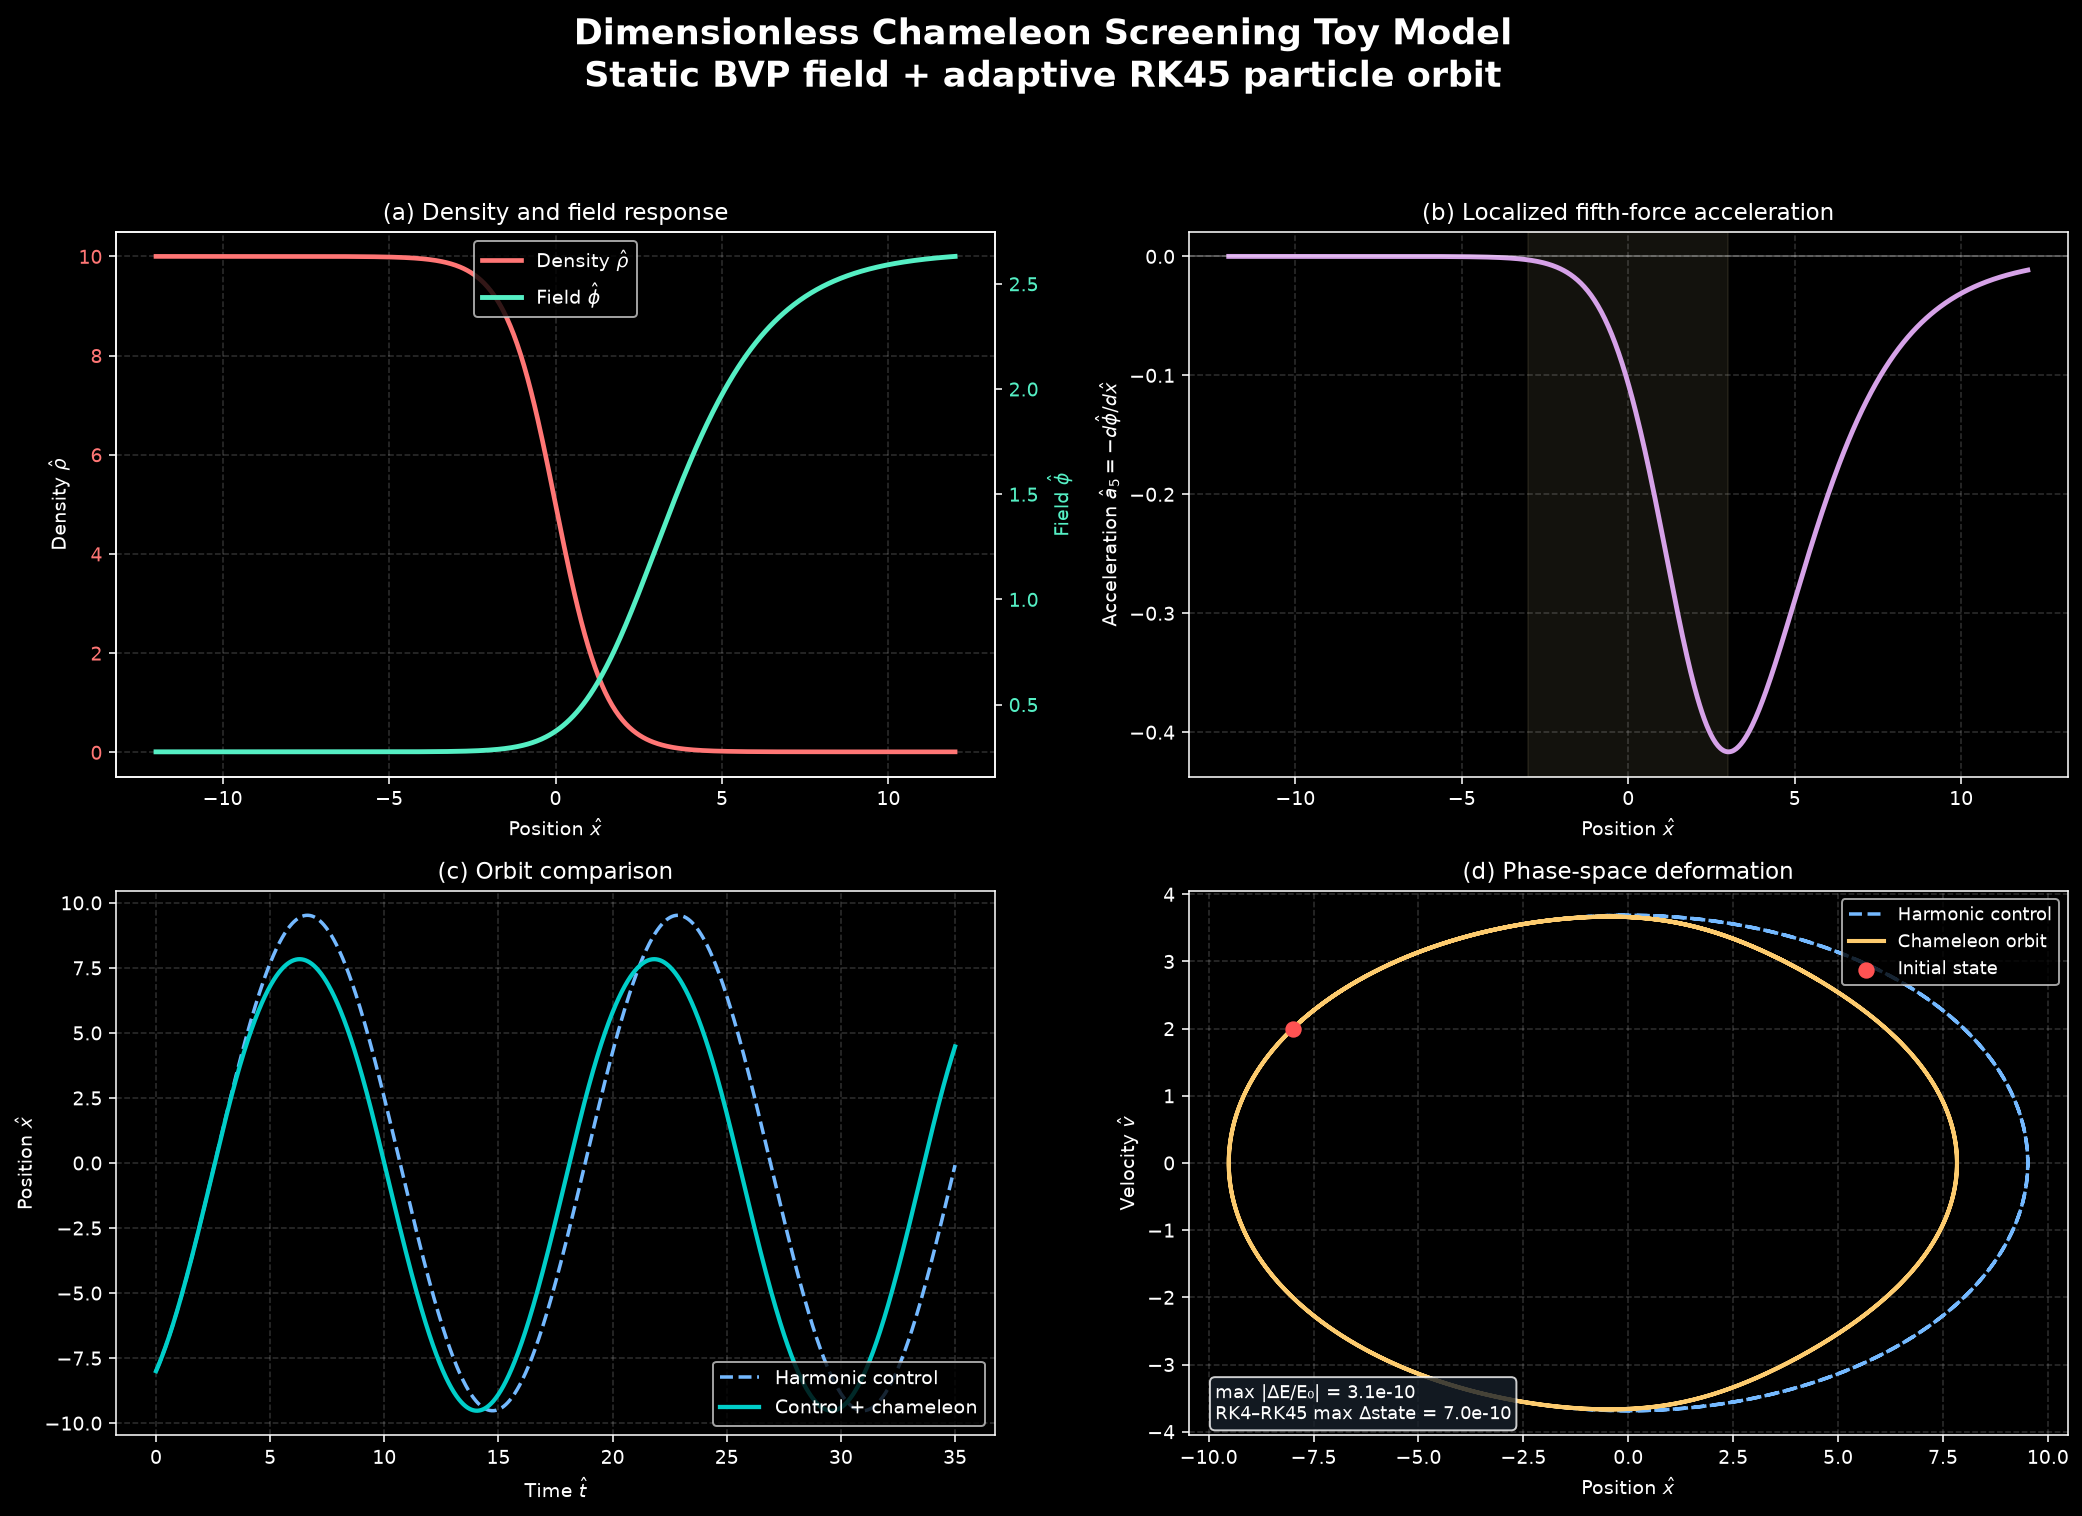
\includegraphics[width=\textwidth]{chameleon_simulation_results.png}
  \end{column}
  \begin{column}{0.31\textwidth}
   \small
   \begin{block}{관측}
    \begin{itemize}\small
     \item $\hat\phi$: $0.2755\rightarrow2.6534$
     \item 제5의 힘은 장이 변하는 전이부에 집중
     \item $-d\hat\phi/d\hat x<0$: 양의 turning point가 감소
     \item 위상 궤적은 비대칭이지만 매끄러운 폐곡선
    \end{itemize}
   \end{block}
   \begin{alertblock}{해석}
    복잡한 모양은 곧 카오스가 아니다. 정적 퍼텐셜에서는
    $E=\hat v^2/2+0.15\hat x^2/2+\hat\phi$가 보존된다.
   \end{alertblock}
  \end{column}
 \end{columns}
\end{frame}

\begin{frame}{6. 결과 II: 구형 고밀도 물체의 screening profile}
 \begin{columns}[T]
  \begin{column}{0.68\textwidth}
   \centering
   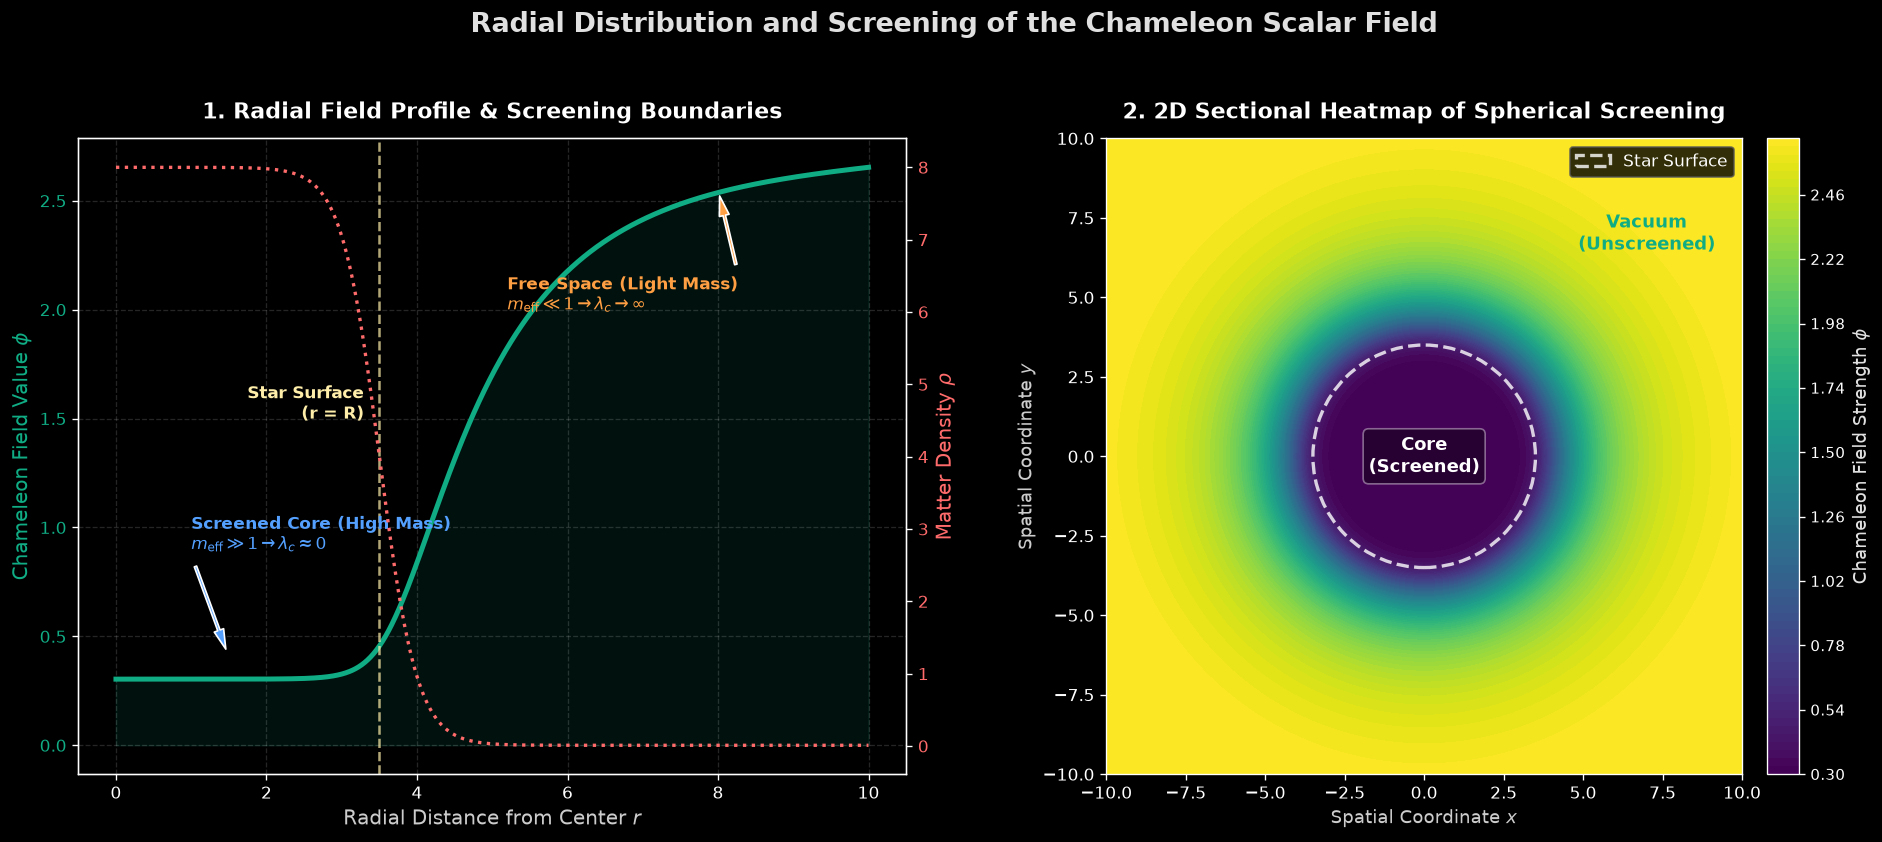
\includegraphics[width=\textwidth]{chameleon_field_distribution.png}
  \end{column}
  \begin{column}{0.30\textwidth}
   \small
   \begin{block}{읽는 법}
    \begin{itemize}\small
     \item 내부: $\phi\simeq\phi_c$, $\nabla\phi\simeq0$
     \item 표면 전이부: 장 구배 형성
     \item 외부: 낮은 환경 밀도에 맞는 값으로 완화
    \end{itemize}
   \end{block}
   \begin{alertblock}{주의}
    색 지도는 장의 공간 분포를 보여준다. 실제 fifth-force 비는 source와 test body의 thin-shell factor를 별도로 포함해야 한다.
   \end{alertblock}
  \end{column}
 \end{columns}
\end{frame}

\begin{frame}[shrink=5]{7. 결과 III: 무작위 밀도장은 정말 chaos를 만드는가?}
 \begin{columns}[T]
  \begin{column}{0.68\textwidth}
   \centering
   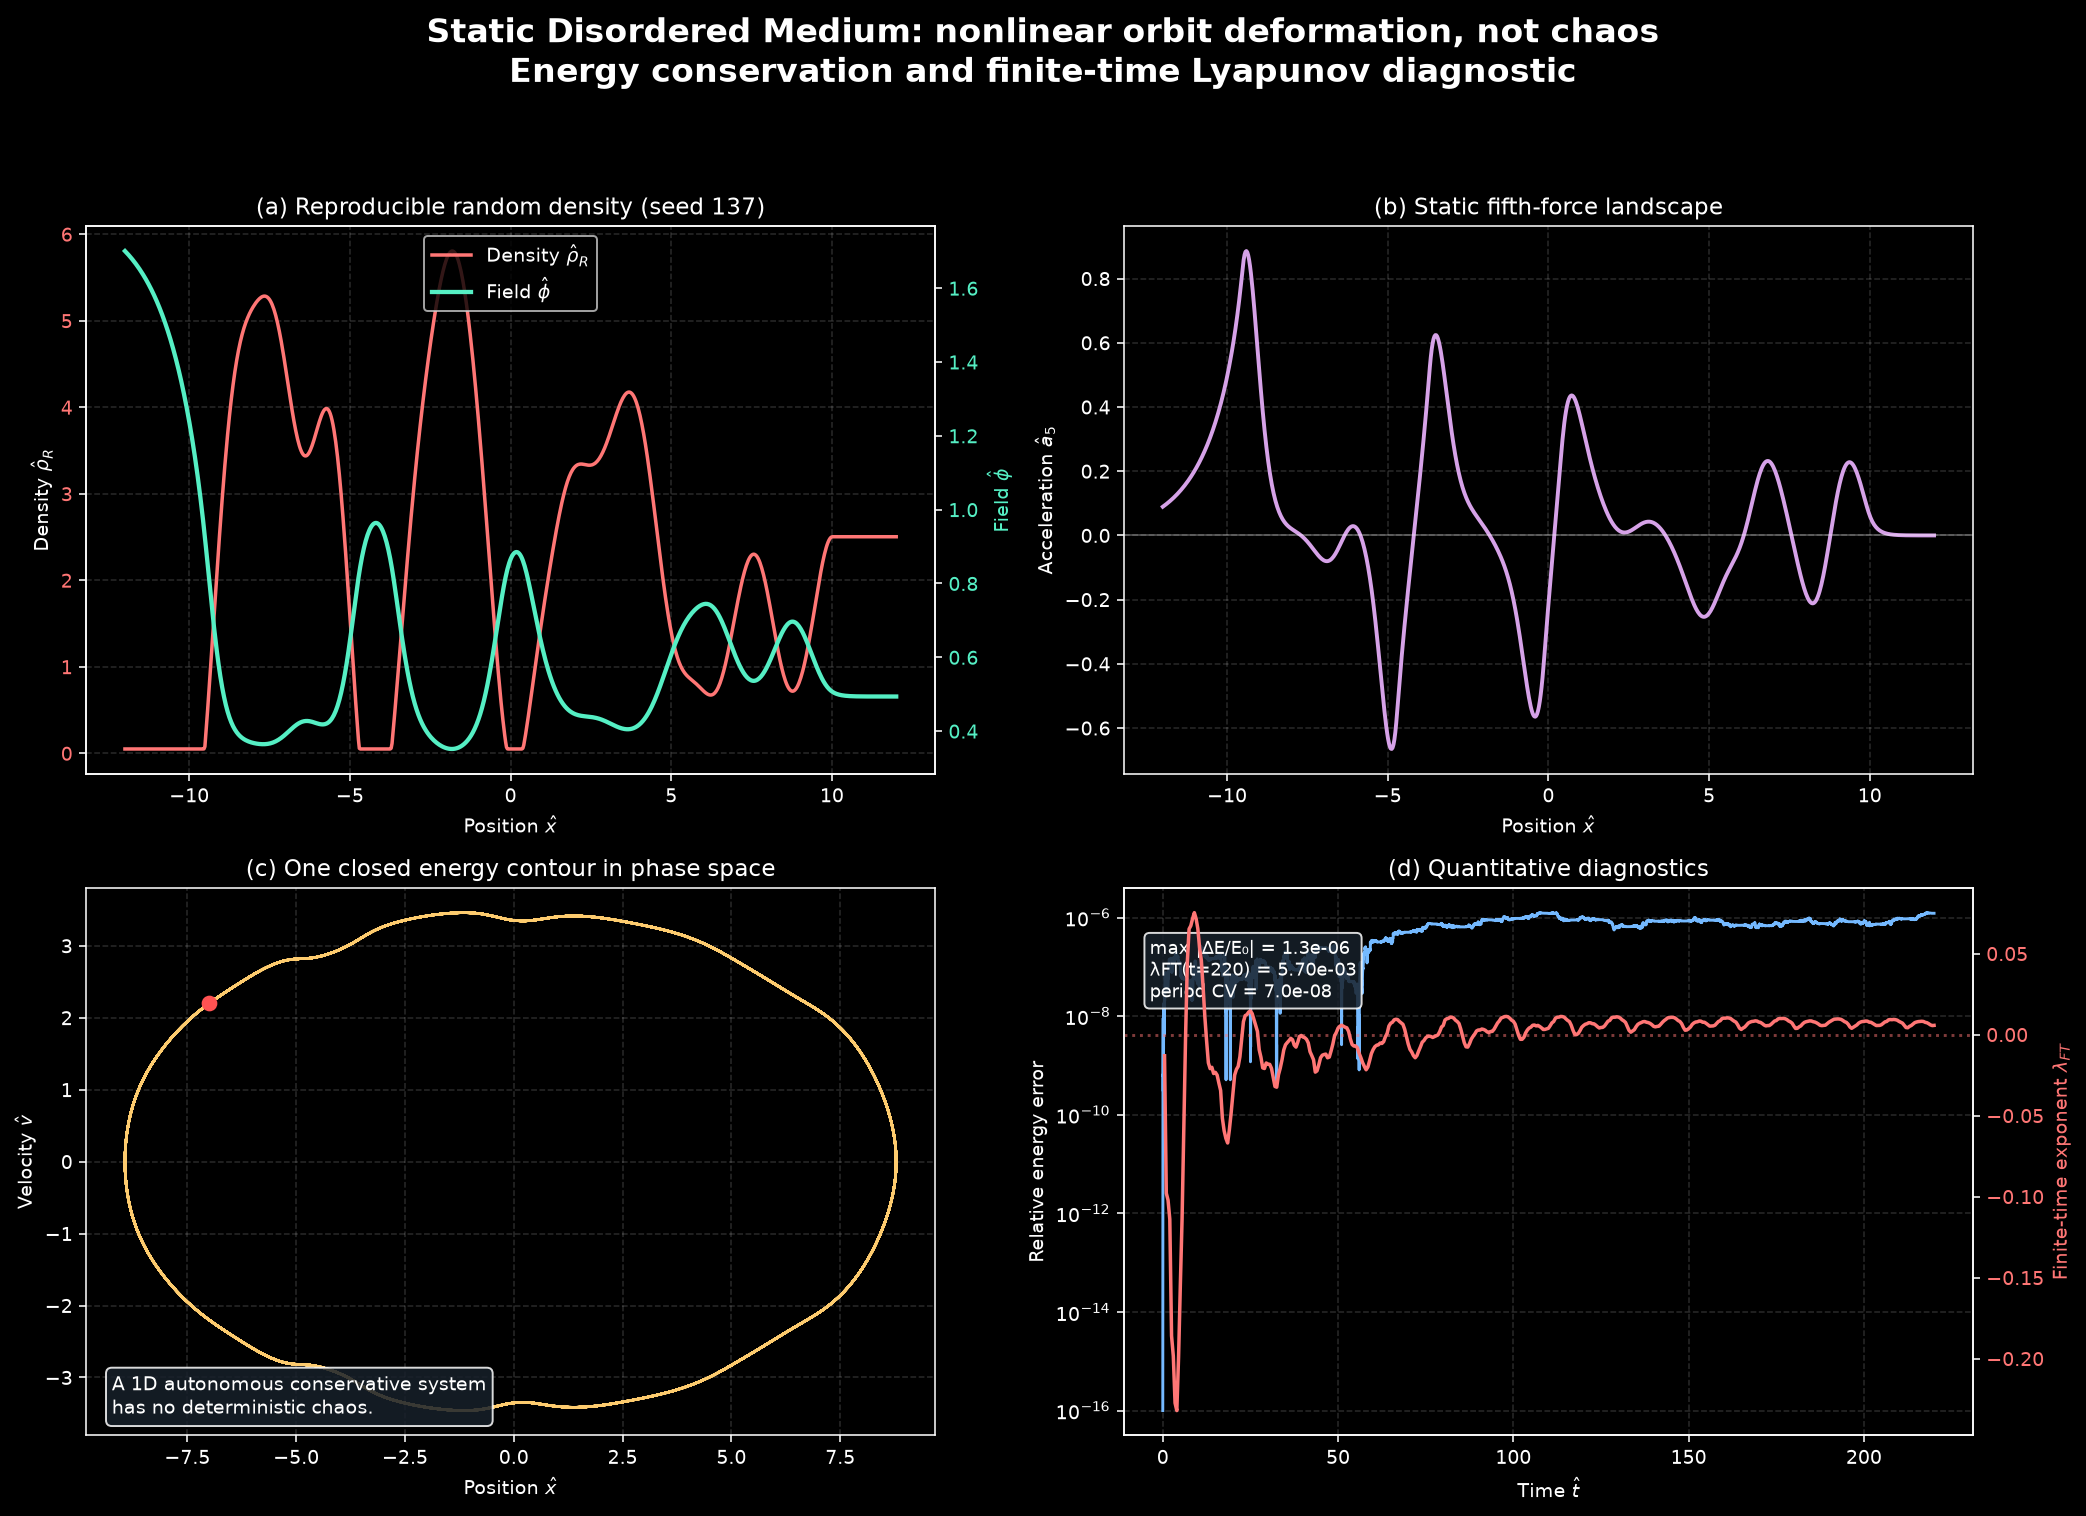
\includegraphics[width=\textwidth]{chameleon_random_medium_results.png}
  \end{column}
  \begin{column}{0.30\textwidth}
   \begin{block}{정량 진단}
    \begin{itemize}\small
     \item 에너지 드리프트 $\sim10^{-6}$
     \item 귀환주기 CV $\sim10^{-7}$
     \item 누적 finite-time Lyapunov 지수는 장시간 양의 상수로 수렴하지 않음
    \end{itemize}
   \end{block}
   \begin{alertblock}{결론 수정}
    1D autonomous conservative system은 적분 가능: \textbf{비선형 궤도 변형은 있으나 chaos 증거는 없다.}
   \end{alertblock}
   \scriptsize 진짜 chaos: 2D 산란, 시간 의존 구동, Poincar\'e section/산란각/Lyapunov spectrum 필요
  \end{column}
 \end{columns}
\end{frame}

\begin{frame}{8. 실험 아이디어: 같은 $\phi(r)$, 다른 센서 응답}
 \begin{columns}[T]
  \begin{column}{0.70\textwidth}
   \centering
   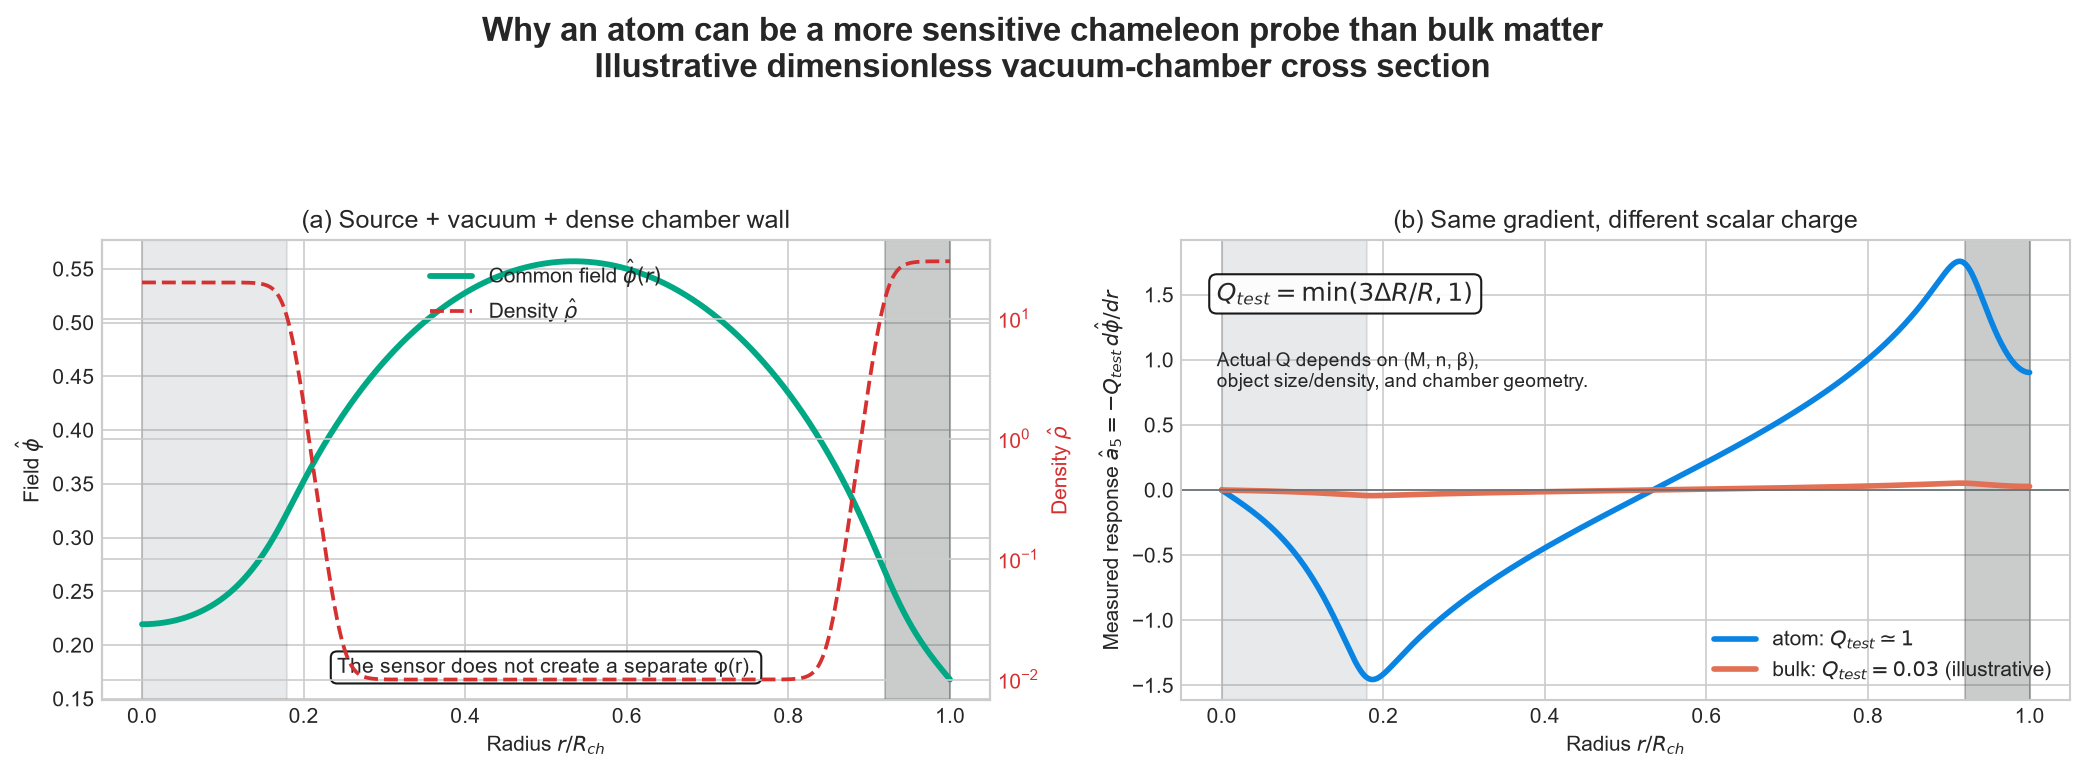
\includegraphics[width=\textwidth]{sensor_detectability.png}
  \end{column}
  \begin{column}{0.28\textwidth}
   \begin{block}{원자 간섭계}
    \begin{enumerate}\small
     \item 초고진공 챔버에 소스 질량 배치
     \item source near/far를 교대
     \item 원자 물질파 위상차로 $a_5$ 탐색
    \end{enumerate}
   \end{block}
   \begin{block}{왜 원자인가?}
    원자는 $Q_{\rm atom}\simeq1$인 비차폐 probe가 될 수 있으나 벌크 센서는 $Q_{\rm bulk}\ll1$로 반응이 억제될 수 있다.
   \end{block}
  \end{column}
 \end{columns}
 \scriptsize 그림의 $Q_{\rm bulk}=0.03$은 원리 설명용이며 특정 실험의 예측값이 아니다.
\end{frame}

\begin{frame}{9. 검출 가능성은 열려 있지만, 실제 파라미터 공간은 강하게 제한된다}
 \begin{columns}[T]
  \begin{column}{0.49\textwidth}
   \begin{block}{실험실}
    \begin{itemize}
     \item Hamilton et al. (2015): Cs atom interferometer로 screened dark-energy 모형 제한
     \item Sabulsky et al. (2019): Rb 원자의 비정상 가속도 신호 없음
     \item Yin et al. (2022): levitated sensor로 기본 dark-energy-scale chameleon 모형 강하게 배제
    \end{itemize}
   \end{block}
  \end{column}
  \begin{column}{0.49\textwidth}
   \begin{block}{천체물리학}
    \begin{itemize}
     \item 은하의 환경별 screening 차이
     \item lensing mass와 dynamical mass 비교
     \item 실제 cosmic-void profile 연구: 선택한 허용 모형에서 $a_\phi/a_N\sim10^{-6}$--$10^{-5}$, 깊이와 내부 구배가 핵심
    \end{itemize}
   \end{block}
  \end{column}
 \end{columns}
 \begin{alertblock}{정확한 결론}
  ``$\beta\sim1$이 허용된다''가 아니라, $(M,n,\beta)$와 환경/기하를 고정한 뒤 해당 exclusion plot에서 판정해야 한다.
 \end{alertblock}
 \scriptsize Sources: Science 349, 849 (2015); PRL 123, 061102 (2019); Nat. Phys. 18, 1181 (2022); JCAP 11, 056 (2022).
\end{frame}

\begin{frame}{10. 결론: 무엇을 보였고, 무엇은 아직 보이지 않았는가?}
 \begin{columns}[T]
  \begin{column}{0.48\textwidth}
   \begin{block}{확인한 것}
    \begin{itemize}
     \item 밀도에 따른 $m_{\rm eff}$와 $\lambda_c$ 변화
     \item BVP 장 해가 만드는 국소 fifth-force 구배
     \item RK45/RK4/해석해/에너지 보존의 일관성
     \item atom vs bulk sensor의 scalar-charge 차이
    \end{itemize}
   \end{block}
  \end{column}
  \begin{column}{0.48\textwidth}
   \begin{alertblock}{남은 과제}
    \begin{itemize}
     \item SI 또는 자연단위로 $(M,n,\beta)$ 완전 지정
     \item 실제 3D 챔버와 source/test screening 계산
     \item 실험 exclusion contour와 수치 비교
     \item chaos 연구는 2D/시간 의존 모형으로 확장
    \end{itemize}
   \end{alertblock}
  \end{column}
 \end{columns}
 \vspace{0.35cm}
 \centering
 \textcolor{TealAccent}{\Large\bfseries Reproducible code and metrics}\par
 \href{https://github.com/Lasqui-Ponto/Mechanics_Term_Project}{https://github.com/Lasqui-Ponto/Mechanics\_Term\_Project}
\end{frame}

\begin{frame}[plain]
 \begin{center}
  \color{NavyDark}
  \vspace{1.2cm}
  \Huge\textbf{Thank You}\\[0.8cm]
  \large Questions and criticism are welcome.\\[0.5cm]
  \small\href{https://github.com/Lasqui-Ponto/Mechanics_Term_Project}{Source code, figures, and verification metrics}
 \end{center}
\end{frame}

\end{document}
